
Similar to the analysis of additive error models in Chapter \ref{chap:phase-transitions}, we will work with triangular arrays of chi-square models \eqref{eq:model-chisq} indexed by $p$.
We adopt the same parametrization for the sparsity of the non-centrality parameter vectors $\lambda = \lambda_p$,
\begin{equation} \label{eq:signal-sparsity}
    |S_p| = \left\lfloor p^{1-\beta} \right\rfloor, \quad \beta\in(0,1]
\end{equation}
where $\beta$ parametrizes the problem sparsity.
The closer $\beta$ is to 1, the sparser the support $S_p$; conversely, when $\beta$ is close to 0, the support is dense with many non-null signals.

We parametrize the range of the non-zero and perhaps unequal signals in the chi-square model with
\begin{equation} \label{eq:signal-size}
    \underline{\Delta} = 2\underline{r}\log{p}
    \le \lambda(i) \le
    \overline{\Delta} = 2\overline{r}\log{p}, \quad \text{for all}\;\;i\in S_p,
\end{equation}
for some constants $0<\underline{r}\le\overline{r}\le+\infty$.

\subsection{The exact support recovery problem}
\label{subsec:exact-support-recovery-chisq}

The first main result characterizes the phase transition phenomenon in the exact support recovery problem under the chi-square model.

\begin{theorem} \label{thm:chi-squared-exact-boundary}
Consider the high-dimensional chi-squared model \eqref{eq:model-chisq} with signal sparsity and size as described in \eqref{eq:signal-sparsity} and \eqref{eq:signal-size}.
The function 
\begin{equation} \label{eq:exact-boundary-chisquared}
    g(\beta) = \left(1 + \sqrt{1-\beta}\right)^2
\end{equation}
characterizes the phase transition of exact support recovery problem.
Specifically, if $\underline{r} > {{g}}(\beta)$, then Bonferroni's, Sid\'ak's, Holm's, and Hochberg's procedures with slowly vanishing (see Definition \ref{def:slowly-vanishing}) nominal FWER levels all achieve asymptotically exact support recovery in the sense of \eqref{eq:support-recovery-success}. 

Conversely, if $\overline{r} < {{g}}(\beta)$, then for any thresholding procedure $\widehat{S}_p$, we have $\P[\widehat{S}_p=S_p]\to0$.
Therefore, in view of Lemma \ref{lemma:risk-exact-recovery-probability}, exact support recovery asymptotically fails for all thresholding procedures in the sense of \eqref{eq:support-recovery-failure}.
\end{theorem}

% \begin{figure}
%   \begin{center}
%     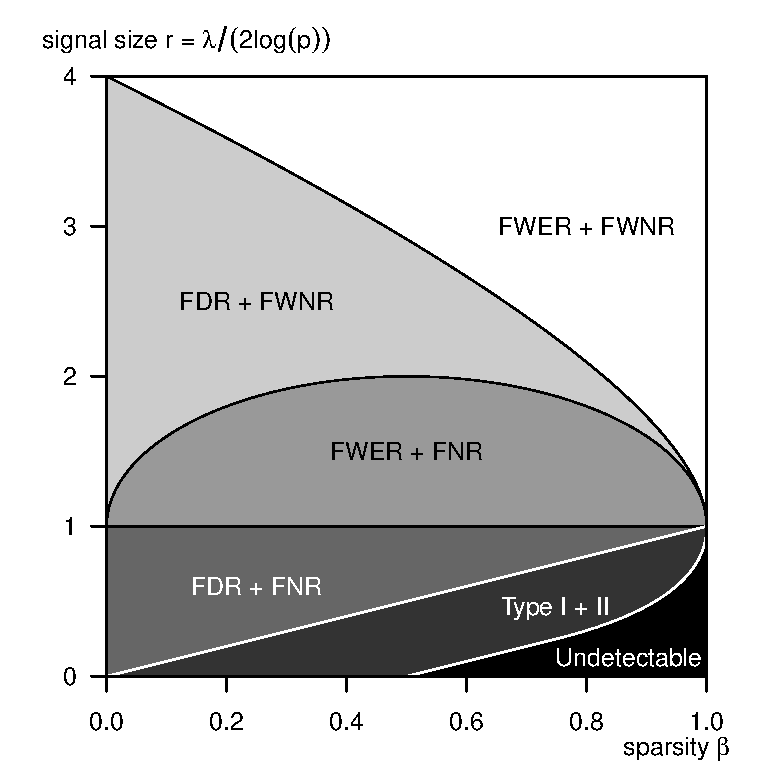
\includegraphics[width=0.7\textwidth]{./pics/phase_diagram_chisquared_ALL_boundaries.eps}
%   \end{center}
%    \caption{The phase diagram for the high-dimensional chi-square model \eqref{eq:model-chisq}, illustrating the boundaries of the exact support recovery (FWER + FWNR; top curve; Theorem \ref{thm:chi-squared-exact-boundary}), the approximate-exact support recovery (FDR + FWNR; second curve from top; Theorem \ref{thm:chi-squared-approx-exact-boundary}), the exact-approximate support recovery (FWER + FNR; horizontal line $r=1$; Theorem \ref{thm:chi-squared-exact-approx-boundary}), and the approximate support recovery problems (FDR + FNR; tilted line $r=\beta$; Theorem \ref{thm:chi-squared-approx-boundary}). The signal detection problem (type I + type II errors of the global test; lower curve) was studied in Donoho and Jin (2004). In each region of the diagram and above, the annotated statistical risk can be made to vanish, as dimension $p$ diverges. Conversely, the risks has liminf at least one. All boundaries are unaffected by the degree-of-freedom. All boundaries are identical to those in the Gaussian additive error model \eqref{eq:model-additive} under one-side alternatives; c.f., results in Section \ref{sec:additive-error-model-boundaries}.}
%    \label{fig:phase-chi-squared}
% \end{figure}


The procedures listed in Theorem \ref{thm:chi-squared-exact-boundary} were reviewed in Section \ref{sec:statistical-procedures}. 
Proof of the theorem can be found in Section \ref{subsec:proof-chi-squared-exact-boundary}. 
% The boundary \eqref{eq:exact-boundary-chisquared} is plotted in Figure \ref{fig:phase-chi-squared}.

It is evident that the exact support recovery boundary \eqref{eq:exact-boundary-chisquared} coincides with that in parallel results for the Gaussian additive error models \eqref{eq:model-additive} in Chapter \ref{chap:phase-transitions}.
Implications of these results will be discussed in Section \ref{subsec:one-vs-two-sided} below.

\begin{remark} \label{rmk:strong-classification-boundary-2}
Theorem \ref{thm:chi-squared-exact-boundary} predicts that the asymptotic boundaries are the same for all values of the parameter $\nu$.
In simulations (Section \ref{sec:numerical}), we find this asymptotic prediction to be quite accurate for $\nu\le3$ even in moderate dimensions ($p=100$). 
For $\nu>3$, the phase transitions take place somewhat above the boundary ${g}$.
The behavior is qualitatively similar for the other three phase transitions (see Theorems \ref{thm:chi-squared-exact-approx-boundary}, \ref{thm:chi-squared-approx-boundary}, and \ref{thm:chi-squared-approx-exact-boundary} below).
\end{remark}

\subsection{The exact-approximate support recovery problem}
\label{subsec:exact-approx-support-recovery-chisq}

The next theorem describes the phase transition in the exact-approximate support recovery problem.

\begin{theorem} \label{thm:chi-squared-exact-approx-boundary}
In the context of Theorem \ref{thm:chi-squared-exact-boundary}, 
the function 
\begin{equation} \label{eq:exact-approx-boundary-chisquared}
    \widetilde{g}(\beta) = 1
\end{equation}
characterizes the phase transition of exact-approximate support recovery problem.
Specifically, if $\underline{r} > \widetilde{g}(\beta)$, then the procedures listed in Theorem \ref{thm:chi-squared-exact-boundary} with slowly vanishing nominal FWER levels achieve asymptotically exact-approximate support recovery in the sense of \eqref{eq:support-recovery-success}. 

Conversely, if $\overline{r} < \widetilde{g}(\beta)$, then for any thresholding procedure $\widehat{S}_p$, the exact-approximate support recovery fails in the sense of \eqref{eq:support-recovery-failure}.
\end{theorem}

Theorem \ref{thm:chi-squared-exact-approx-boundary} is proved in Section \ref{subsec:proof-chi-squared-mix-boundaries}. 


\subsection{The approximate support recovery problem}
\label{subsec:approx-support-recovery-chisq}

Our third main result characterizes the phase transition phenomenon in the approximate support recovery problem in the chi-square model.

\begin{theorem} \label{thm:chi-squared-approx-boundary}
Consider the high-dimensional chi-squared model \eqref{eq:model-chisq} with signal sparsity and size as described in \eqref{eq:signal-sparsity} and \eqref{eq:signal-size}.
The function 
\begin{equation} \label{eq:approx-boundary-chisquared}
    h(\beta) = \beta
\end{equation}
characterizes the phase transition of approximate support recovery problem.
Specifically, if $\underline{r} > {h}(\beta)$, then the \ac{BH} procedure $\widehat{S}_p$ (defined in Section \ref{sec:statistical-procedures}) with slowly vanishing (see Definition \ref{def:slowly-vanishing}) nominal FDR levels achieves asymptotically approximate support recovery in the sense of \eqref{eq:support-recovery-success}. 

Conversely, if $\overline{r} < {h}(\beta)$, then approximate support recovery asymptotically fails in the sense of \eqref{eq:support-recovery-failure} for all thresholding procedures.
\end{theorem}

Theorem \ref{thm:chi-squared-approx-boundary} is proved in Section \ref{subsec:proof-chi-squared-mix-boundaries} below. 


\subsection{The approximate-exact support recovery problem}
\label{subsec:aprox-exact-support-recovery-chisq}

A counterpart of Theorem \ref{thm:Gaussian-error-approx-exact-boundary} also holds in the chi-square models.

\begin{theorem} \label{thm:chi-squared-approx-exact-boundary}
In the context of Theorem \ref{thm:chi-squared-approx-boundary}, the function 
\begin{equation} \label{eq:approx-exact-boundary-chisquared}
    \widetilde{h}(\beta) = \left(\sqrt{\beta} + \sqrt{1-\beta}\right)^2
\end{equation}
characterizes the phase transition of approximate-exact support recovery problem.
Specifically, if $\underline{r} > \widetilde{h}(\beta)$, then the Benjamini-Hochberg procedure with slowly vanishing nominal FDR levels achieves asymptotically approximate-exact support recovery in the sense of \eqref{eq:support-recovery-success}. 

Conversely, if $\overline{r} < \widetilde{h}(\beta)$, then for any thresholding procedure $\widehat{S}_p$, the approximate-exact support recovery fails in the sense of \eqref{eq:support-recovery-failure}.
\end{theorem}

Theorem \ref{thm:chi-squared-approx-exact-boundary} is proved in Section \ref{subsec:proof-chi-squared-exact-boundary}. 

Notice that all phase transitions boundaries are identical to those in the Gaussian additive error model \eqref{eq:model-additive} under one-side alternative.
We refer readers to Figure \ref{fig:phase-Gaussian-errors} in Section \ref{sec:additive-error-model-boundaries} for a visualization of the results in Theorems \ref{thm:chi-squared-exact-boundary} through \ref{thm:chi-squared-approx-exact-boundary}.

\medskip

The all four Theorems so far focus only on the idealized models \eqref{eq:model-chisq} where statistics are \emph{independent}.
Support recovery problems under dependent observations remain to be explored.
Recall in Chapter \ref{chap:phase-transitions} we showed that the boundary for the exact support recovery problem in the additive error model \eqref{eq:model-additive} continues to hold even under severe dependence and general distributional assumptions.
We conjecture that similar results would also hold, under classes of dependence structures that are ``not too different from independence'', in the chi-square models.
As an example, in the GWAS application, dependence among the genetic markers at different locations (known as linkage disequilibrium) decay as a function of their physical distances on the genome \citep{bush2012genome}, resulting in locally dependent test statistics.
It would be of great interest to extend the current theory to cover important dependence structures that arise in such applications.


\subsection{Comparison of one- versus two-sided alternatives in additive error models}
\label{subsec:one-vs-two-sided}


% $\mathrm{risk}^{\mathrm{EA}}$ and $\mathrm{risk}^{\mathrm{AE}}$.
As alluded to in Section \ref{sec:motivation-chisq} in the introduction, we draw explicit comparisons between the one-sided and two-sided alternatives in Gaussian additive error models \eqref{eq:model-additive}.
% The exact, and the approximate support recovery problems in the additive error model \eqref{eq:model-additive} under standard Gaussian errors have been studied in \cite{gao2018fundamental} and \cite{arias2017distribution}, respectively. 

The exact support recovery problem in the dependent Gaussian additive error model \eqref{eq:model-additive} was studied in Chapter \ref{chap:phase-transitions}, with parametrization of sparsity identical to that in \eqref{eq:signal-sparsity}, whereas the range of the non-zero (and perhaps unequal) mean shifts $\mu(i)$ was parametrized as 
\begin{equation*}
    \underline{\Delta} = \sqrt{2\underline{r}\log{p}}
    \le \mu(i) \le
    \overline{\Delta} = \sqrt{2\overline{r}\log{p}}, \quad \text{for all}\;\;i\in S_p,
\end{equation*}
for some constants $0<\underline{r}\le\overline{r}\le+\infty$.
Under this one-sided alternative, a phase transition in the $r$-$\beta$ plane was described, where the boundary was found to be identical to \eqref{eq:exact-boundary-chisquared} in Theorem \ref{thm:chi-squared-exact-boundary} for the chi-square models \eqref{eq:model-chisq-Chapter6}. 

As discussed in Section \ref{sec:motivation-chisq}, support recovery problems in the chi-square model with $\nu=1$ correspond to the support recovery problems in 
the additive model under two-sided alternatives. This implies that the asymptotic signal size requirements are identical between the two-sided alternative and its 
one-sided counterpart, in order to achieve exact support recovery. As we shall see in numerical experiments (in Section \ref{sec:numerical} below), the difference 
is not very pronounced even in moderate dimensions, and vanishes as $p\to\infty$, in accordance with Theorem \ref{thm:chi-squared-exact-boundary}.

\medskip

Comparisons can also be drawn in the approximate, approximate-exact, and exact approximate support recovery problems between the two types of alternatives.

Specifically, the approximate support recovery problem in the Gaussian additive error model \eqref{eq:model-additive} under one-sided alternatives exhibits a phase transition phenomenon characterized by a boundary that coincides with \eqref{eq:approx-boundary-chisquared} in Theorem \ref{thm:chi-squared-approx-boundary}.
Similar to the exact support recovery problem, this indicates vanishing difference in the difficulties of the two types alternatives in approximate support recovery problems.

Comparing Theorems \ref{thm:chi-squared-exact-approx-boundary} to \ref{thm:Gaussian-error-exact-approx-boundary} and Theorems \ref{thm:chi-squared-approx-exact-boundary} to \ref{thm:Gaussian-error-approx-exact-boundary}, we see that the phase transition boundaries under the two types of alternatives are also identical in the exact-approximate and approximate-exact support recovery problems.
The additional uncertainty in the two-sided alternatives do not call for larger signal sizes asymptotically in these problems.

\medskip

To complete the comparisons, we point out that the phase transition boundaries for the sparse signal {detection} problem in the two types of alternatives are both identical to \eqref{eq:detection-boundary-large-signals}. This was analyzed in \cite{donoho2004higher}.




